
\section{Human Brain Project - brain analytics}


\subsection{The Project}

The Human Brain Project aims to acquire a better understanding of
the human brain by modeling it as a whole. One sub task of this project
is to build a 3d model of the human brain.

The brain analytics data set provides images of different cross sections
of a brain and each pixel is labeled whether it belongs to the cross
section or not. Labeling a whole brain takes a huge amount of time
and resources. So instead of labeling new images by hand, this data
is used to build a model that automatically classifies a pixel. If
this classification is good enough, the predicted 2d brain parts should
be used to rebuild a 3d model of a human brain. 

\begin{figure}[h] \centering 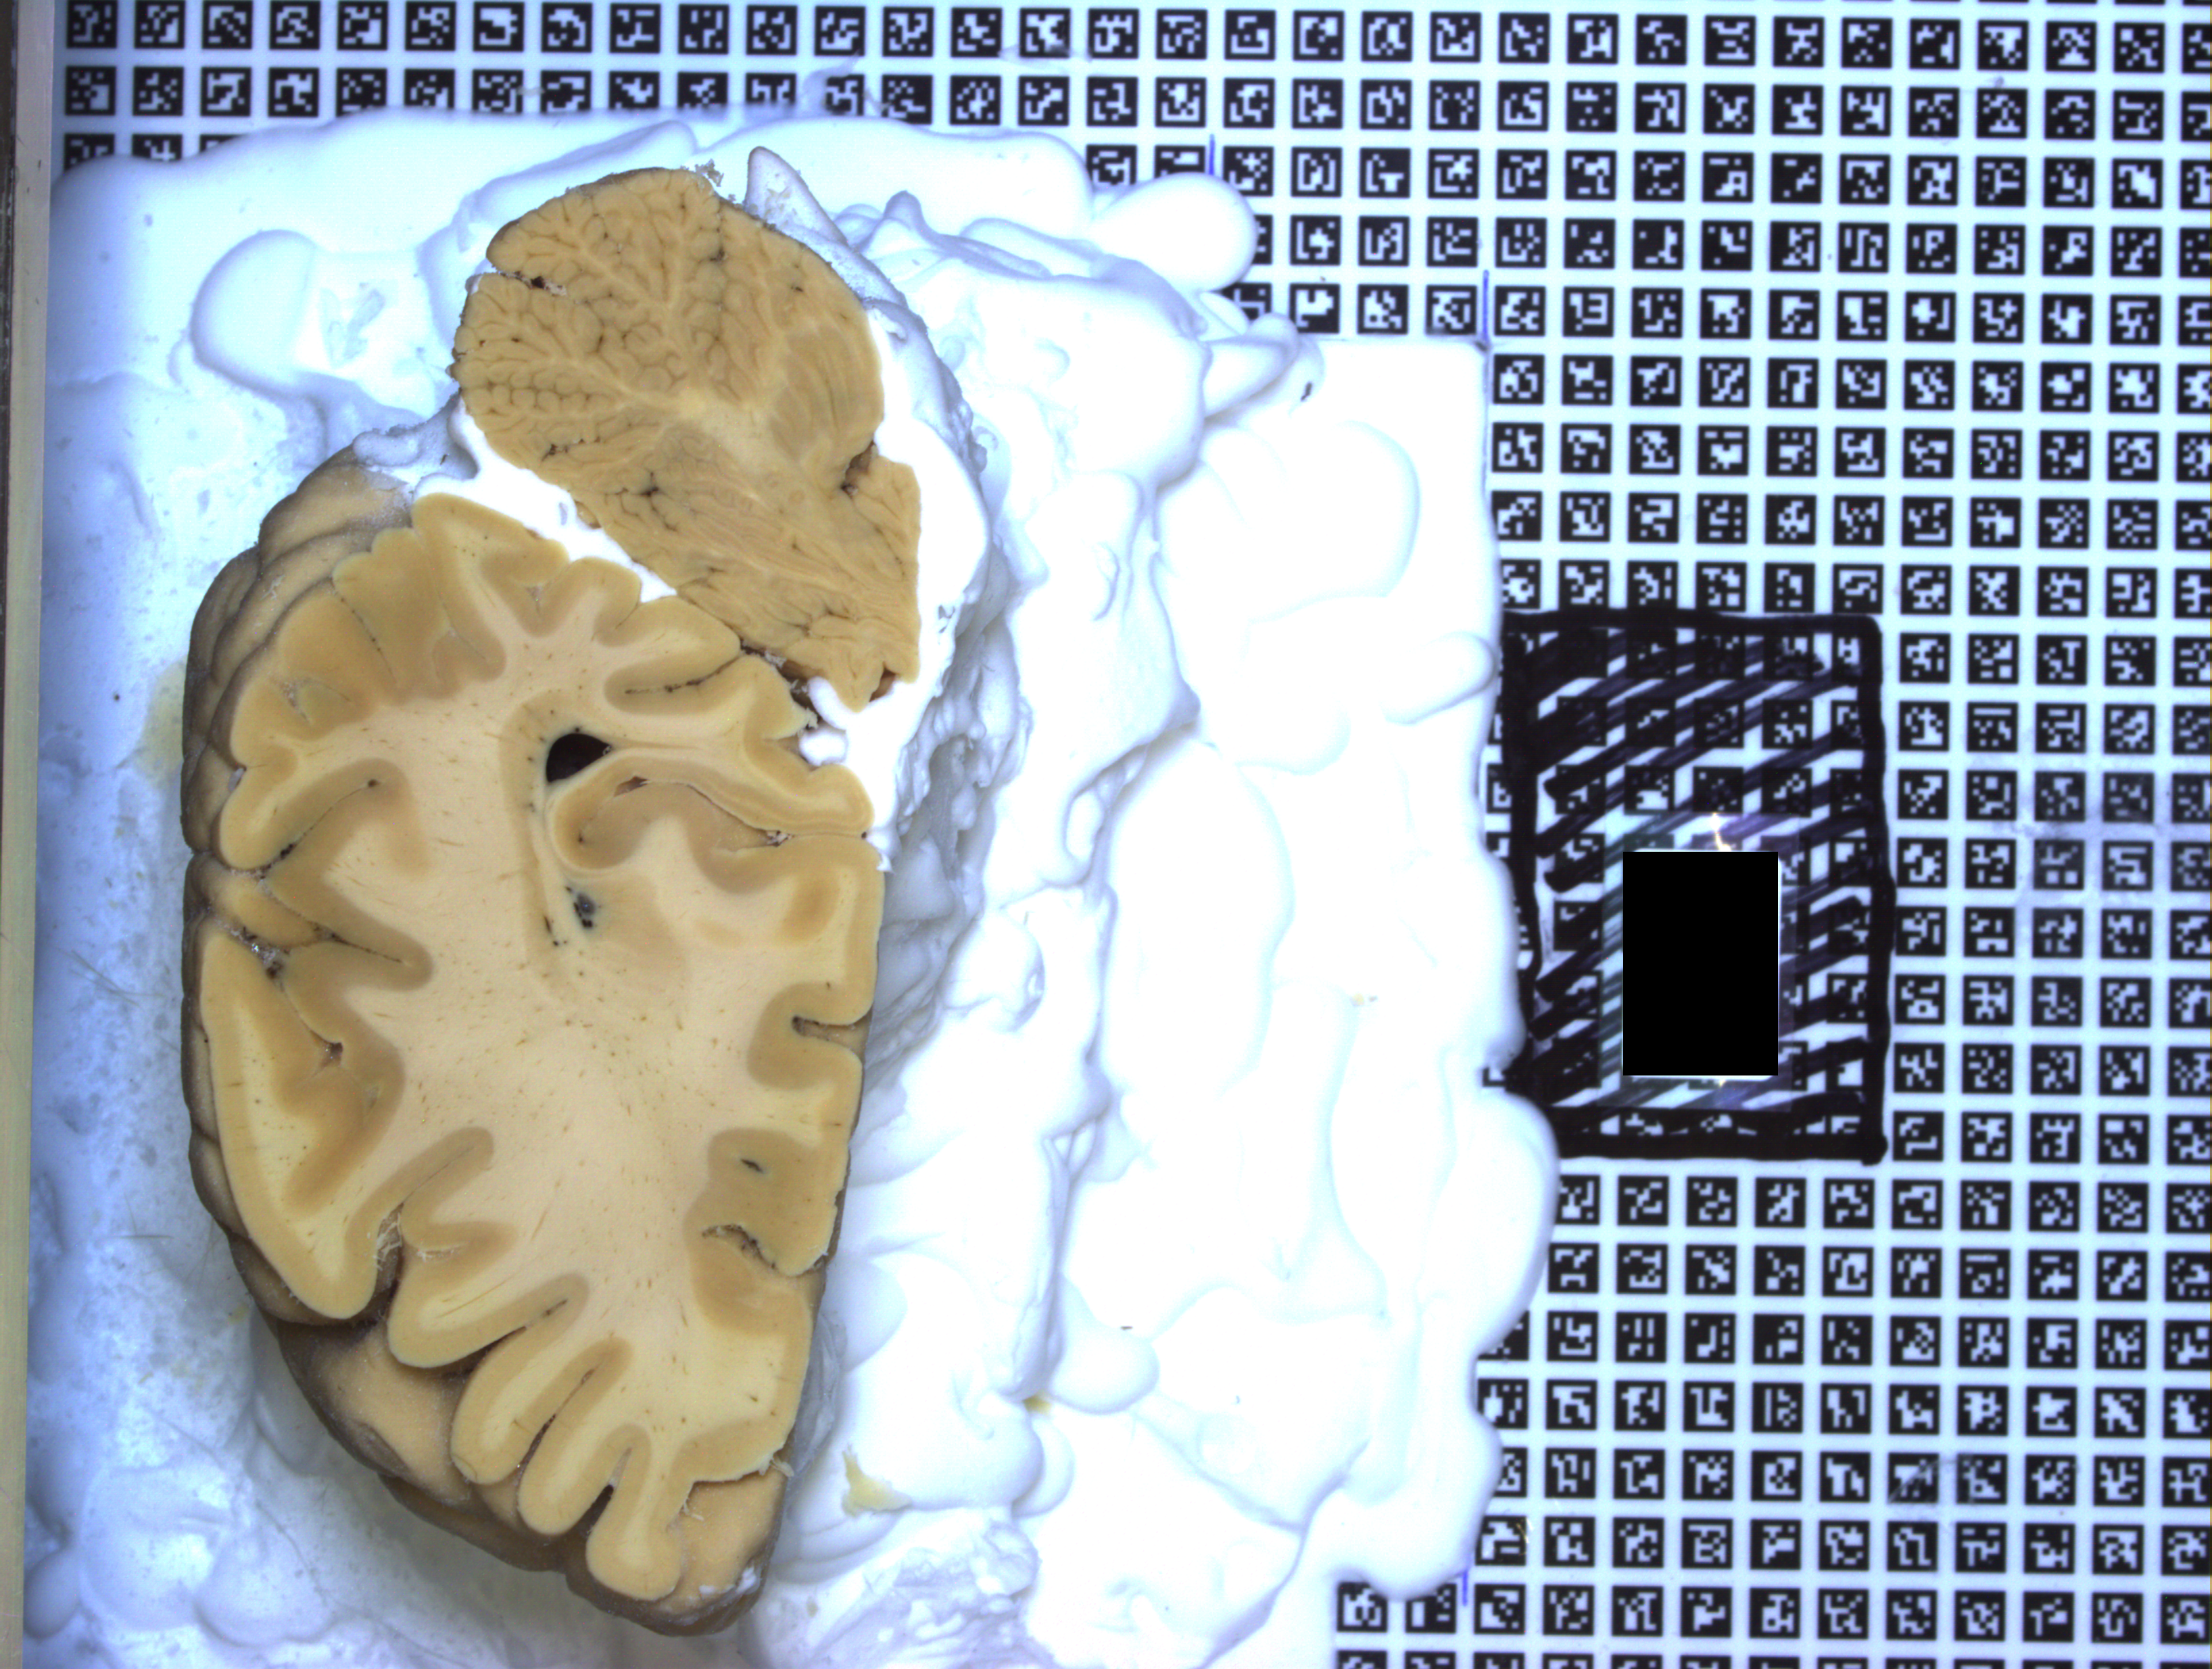
\includegraphics[width=0.6\linewidth]{graphics/original603} \caption{An image of a cross section of a human brain} \label{fig:original603} \end{figure}
